\chapter{Coloring}
Rishnak was eager to meet Ajur, as he was impressed with his logical reasoning. Finally he found Ajur walking along with Jura. Rishnak caught up with Ajur. Rishnak asked Ajur whether Ajur likes coloring. Ajur responded that he really enjoyed coloring and it had a calming effect on him.

Rishnak was glad to hear that. He said that there is also a way to color the vertices of a graph. Rishnak added that a proper vertex coloring is coloring of vertices such that no adjacent vertices (i.e., vertices connected by an edge) can get the same color. To make it more interesting the question is what is the smallest number of colors to properly vertex color a graph. 
Rishnak showed an example of proper coloring of a graph \ref{10g1} with 4 colors. Ajur jumped up and down and said that he could color it three colors and showed his coloring in \ref{10g2}.
\begin{figure}[h]
\begin{center}
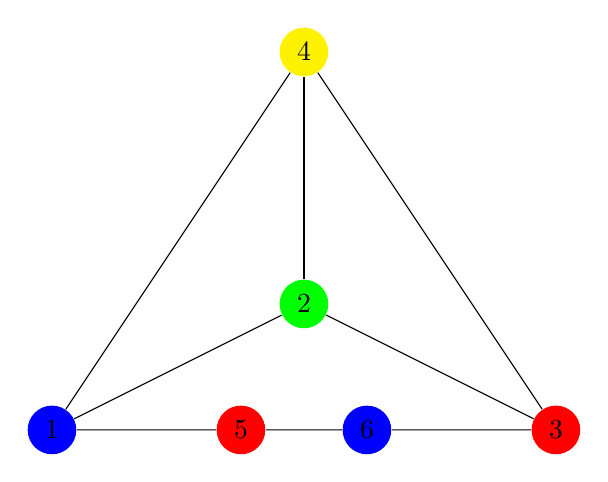
\begin{tikzpicture}
  [scale=.8,auto=left,every node/.style={circle}]
  \node (n1)[fill=blue] at (-1,7) {1};
  \node (n2)[fill=green] at (3,9)  {2};
  \node (n3)[fill=red] at (7,7)  {3};
  \node (n4)[fill=yellow] at (3,13)  {4};
  \node (n5)[fill=red] at (2,7) {5};
  \node (n6)[fill=blue] at (4,7) {6};
 \foreach \from/\to in {n1/n2,n2/n3,n2/n4,n1/n4,n3/n4,n1/n5,n5/n6,n6/n3}
    \draw (\from) -- (\to);
\end{tikzpicture}
\caption{ Proper Coloring the vertices of a graph with 4 colors}\label{10g1}
\end{center}
\end{figure}

\begin{figure}[h]
\begin{center}
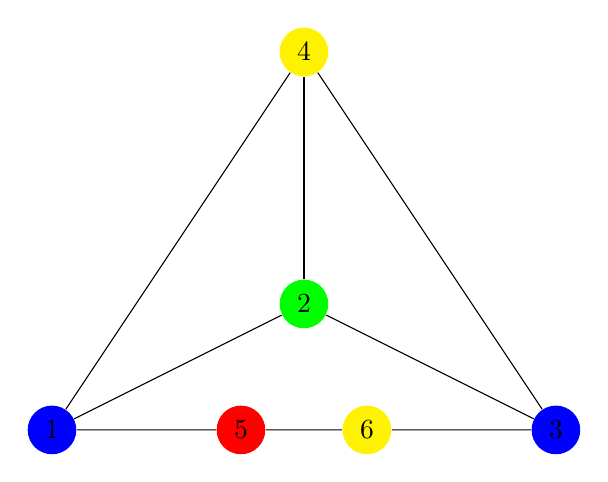
\begin{tikzpicture}
  [scale=.8,auto=left,every node/.style={circle}]
  \node (n1)[fill=blue] at (-1,7) {1};
  \node (n2)[fill=green] at (3,9)  {2};
  \node (n3)[fill=blue] at (7,7)  {3};
  \node (n4)[fill=yellow] at (3,13)  {4};
  \node (n5)[fill=red] at (2,7) {5};
  \node (n6)[fill=yellow] at (4,7) {6};
 \foreach \from/\to in {n1/n2,n2/n3,n2/n4,n1/n4,n3/n4,n1/n5,n5/n6,n6/n3}
    \draw (\from) -- (\to);
\end{tikzpicture}
\caption{ Proper Coloring the vertices of a graph with 3 colors colors}\label{10g2}
\end{center}
\end{figure}

Ajur further stated that 3 colors are needed a vertices 1, 2 and 4 are mutually adjacent and those vertices need 3 different colors. 
Rishnak asked Ajur to properly color the graph $K_{3,3}$, a complete bipartite graph. Ajur jumped at the opportunity and showed a 2 coloring of this graph \ref{10g3}
\begin{figure}
\begin{center}
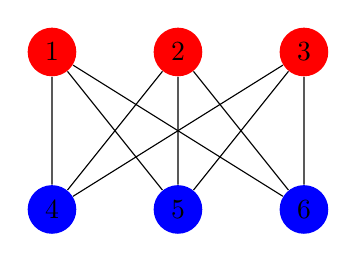
\begin{tikzpicture}
  [scale=.4,auto=left,every node/.style={circle}]
  \node (n1)[fill=red] at (1,7) {1};
  \node (n2)[fill=red] at (5,7)  {2};
  \node (n3)[fill=red] at (9,7) {3};
  \node (n4) [fill=blue] at (1,2)  {4};
  \node (n5) [fill=blue] at (5,2) {5};
  \node (n6)[fill=blue] at (9,2)  {6};
 
  
   \foreach \from/\to in {n1/n6,n1/n4,n1/n5,n2/n6,n2/n4,n2/n5,n3/n4,n3/n5,n3/n6}
    \draw (\from) -- (\to);
    \end{tikzpicture}
\caption{ Two coloring of a Bipartite Graph with 6 vertices and 9 edges, denoted by $K_{3,3}$}\label{10g3}
\end{center}
\end{figure}

Ajur further said that any bipartite graph Vertices are partitioned into two sets $A$ and $B$ and the edges always go from one set, $A$, to the other set, $B$. Ajur further stated that all the vertices in $A$ can be colored with one color, say, red and all the vertices in $B$ can be colored with another color, say blue. Since all tress are also bipartite graphs (contains cycles of even length (=0)), trees can be colored with just two colors. He showed an example \ref{10g4}. Coloring of trees reminded Ajur of the beautiful fall colors one sees in the trees!
\begin{figure}
\begin{center}

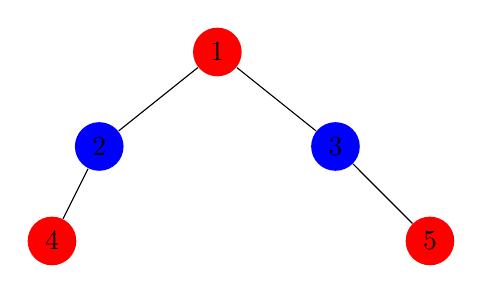
\begin{tikzpicture}
  [scale=.6,auto=left,every node/.style={circle}]
  \node (n1)[fill=red] at (5.5,7) {1};
  \node (n2)[fill=blue] at (3,5)  {2};
  \node (n3)[fill=blue] at (8,5)  {3};
  \node (n4)[fill=red] at (2,3) {4};
  \node (n5)[fill=red] at (10,3)  {5};


  \foreach \from/\to in {n1/n2,n1/n3,n2/n4,n3/n5}
    \draw (\from) -- (\to);

\end{tikzpicture}

\caption{Two coloring of a tree }\label{10g4}
\end{center}
\end{figure}

Map Coloring problem is to color the regions or faces of a planar graph (maps are usually drawn on a plane) so that no two adjacent faces or regions are colored the same.




